%!TEX root=../GaugeCNNTheory.tex


\section{\lr{CNN}های کروی مستقل از مختصات}
\label{sec:instantiations_spherical}

\begin{figure}
    \centering
    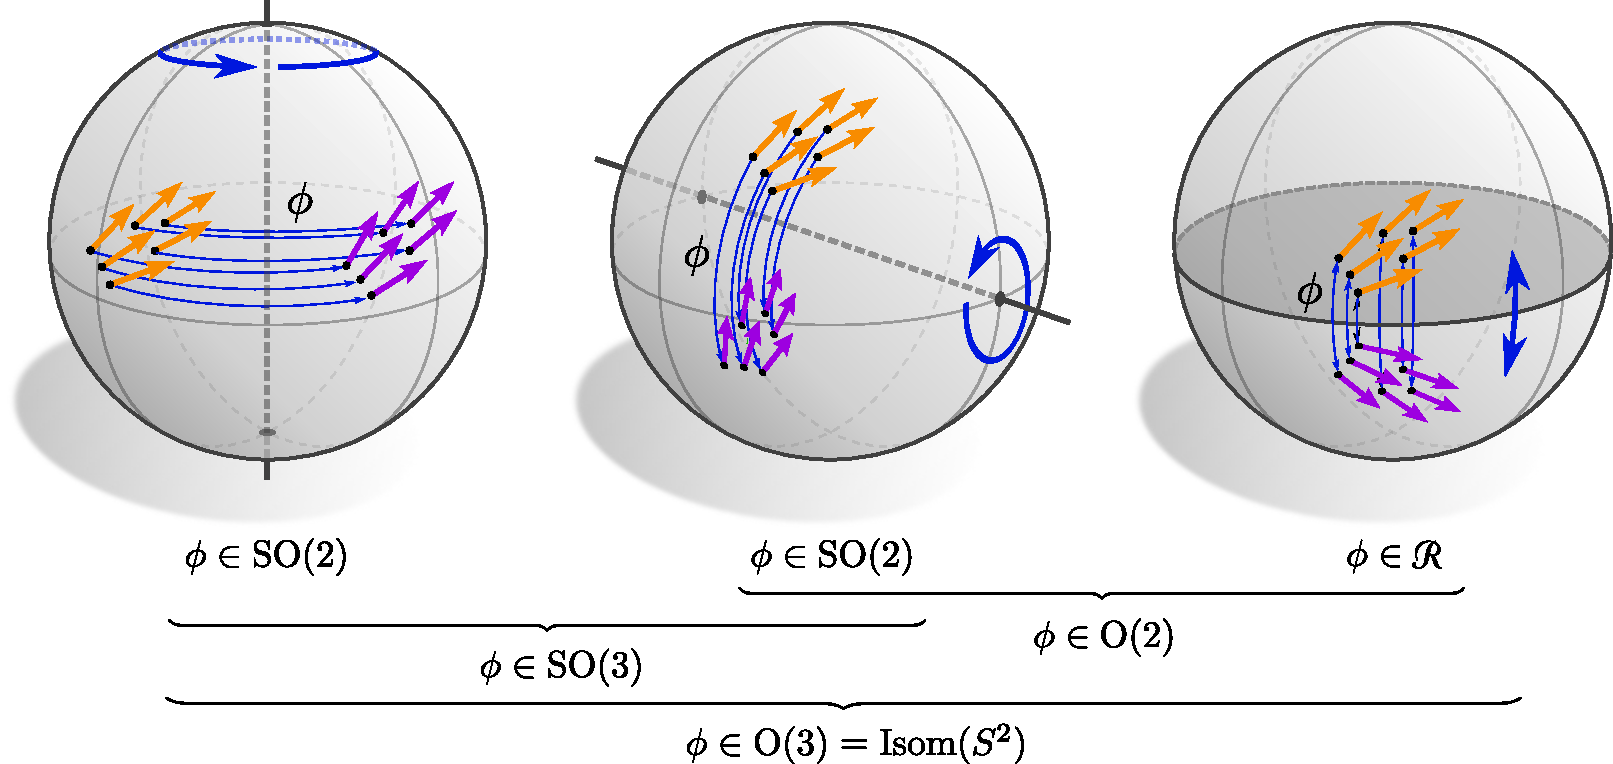
\includegraphics[width=1.\textwidth]{figures/isometry_sphere.pdf}
    \caption{\small
        نمایش گروه ایزومتری کره ۲-بعدی $\Isom(S^2) = \O3$ و زیرگروه‌های مختلف آن.
        می‌توان گروه ایزومتری را متشکل از دوران‌های حافظ جهت در $\Isom_+(S^2) = \SO3$ و بازتاب‌ها $\Flip$ از طریق حاصلضرب مستقیم $\O3 = \SO3 \times \Flip$ در نظر گرفت.
        $\SO3$ به نوبه خود، توسط دوران‌های $\SO2$ حول هر دو محور غیرموازی تولید می‌شود، که در پارامترسازی زاویه اویلر استفاده می‌شود.
        برای زیرگروه‌های مرتبط بیشتر و روابط آنها به متن اصلی مراجعه کنید.
    }
    \label{fig:isometries_sphere}
\end{figure}


فراتر از کانولوشن‌ها در فضاهای اقلیدسی، کانولوشن‌ها روی کره ۲-بعدی $S^2$ از اهمیت عملی بالایی برخوردارند.
کاربردها شامل وظایف بینایی همه‌جانبه، پیش‌بینی جهانی آب و هوا، یا تحلیل تابش زمینه کیهانی است.
کانولوشن‌های کروی به جای هموردایی انتقالی، معمولاً باید هموردای دورانی باشند.
گروه ایزومتری کره $\Isom(S^2) = \O3$ و تجزیه آن به زیرگروه‌های مرتبط‌تر در شکل~\ref{fig:isometries_sphere} به تصویر کشیده شده است.

یک تفاوت عمده بین فضاهای اقلیدسی $\Euc_d$ و کره $S^2$ این است که دومی موازی‌پذیر نیست، یعنی اجازه یک میدان چارچوب سراسری و پیوسته را نمی‌دهد.
تقلیل گروه ساختاری فراتر از $G=\SO2$ از نظر توپولوژیکی مسدود شده است، که به این معنی است که کانولوشن‌های کروی حداقل به کرنل‌های $\SO2$-راهبری‌پذیر نیاز دارند اگر بخواهند پیوستگی میدان‌های ویژگی را حفظ کنند.
$\SO2$-ساختار متناظر، که به طور کامل توسط متریک و جهت‌گیری کره تعیین می‌شود، در شکل~\ref{fig:G_structure_S2_1} نشان داده شده است.
کانولوشن‌های $\GM$ روی این $G$-ساختار ناوردای دورانی سراسری، تضمین می‌شوند که $\IsomSOM = \SO3$-هموردا باشند.

علی‌رغم مانع توپولوژیکی اجتناب‌ناپذیر، بسیاری از نویسندگان \lr{CNN}های کروی را پیشنهاد داده‌اند که از کرنل‌های $\SO2$-راهبری‌پذیر استفاده نمی‌کنند.
رایج‌ترین انتخاب $\{e\}$-ساختار متناظر با چنین کانولوشن‌هایی، میدان چارچوب نشان داده شده در شکل~\ref{fig:G_structure_S2_2} است، که چارچوب‌های مرجع راست‌هنجار آن (معادله~\eqref{eq:spherical_e_structure_frames}) با شبکه مختصاتیِ مختصات کروی تراز شده‌اند.
توجه داشته باشید که این میدان چارچوب دارای تکینگی‌هایی در قطب‌ها است، جایی که کانولوشن‌ها ناپیوسته می‌شوند.
برای تطبیق چنین مدل‌هایی با نظریه ما، به ویژه فرض همواری $G$-ساختارها، آنها باید به عنوان کانولوشن‌هایی روی یک استوانه توپولوژیکی با متریک شبه-کروی توصیف شوند.
گروه ایزومتری این کره سوراخ‌دار $S^2 \backslash \{n,s\}$ بدون قطب‌های $n,s \in S^2$ زیرگروه $\O2$ (شکل~\ref{fig:isometries_sphere} (وسط و راست)) از گروه ایزومتری کامل کره $\O3$ است.
$\{e\}$-ساختار به تصویر کشیده شده توسط دوران‌های سمتی در $\IsomeM = \SO2$ حفظ می‌شود، یعنی دوران حول محور گذرنده از قطب‌ها.

از دیدگاه مهندسی، هر دو رویکرد توجیه خود را دارند:
کاربردهای کاملاً همسانگرد مانند تحلیل تابش زمینه کیهانی به مدل‌های کاملاً $\SO3$-هموردا روی~$S^2$ نیاز دارند.
وظایف یادگیری که با یک محور دوران مرجح همراه هستند، که به عنوان مثال برای زمین یا تصاویر پانوراما با جهت‌های «بالا» و «پایین» مشخص، صادق است، ممکن است از اطلاعات هندسی اضافی کدگذاری شده در $\{e\}$-ساختار بهره‌مند شوند.
نتایج تجربی نشان می‌دهد که در چنین مواردی اغلب مفید است که با ترکیبی از هر دو رویکرد کار شود:
لایه‌های اولیه با کانولوشن‌های کاملاً هموردا می‌توانند از تقارن‌های محلی در داده‌ها بهره‌برداری کنند، در حالی که لایه‌های بعدی با تنها هموردایی سمتی می‌توانند بر اساس محور مرجح، یاد بگیرند که تمایز قائل شوند؛ به بخش ۲.۷ در~\cite{3d_steerableCNNs} مراجعه کنید.


\etocsettocdepth{3}
\etocsettocstyle{}{} % from now on only local tocs
\localtableofcontents


ما با توصیف هندسه کره در بخش~\ref{sec:sphere_geometry} شروع می‌کنیم.
بخش~\ref{sec:spherical_CNNs_fully_equivariant} کانولوشن‌های $\GM$ کروی کاملاً $\SO3$- و $\O3$-هموردا را مورد بحث قرار می‌دهد، که بر $\SO2$- یا $\O2$-ساختارها همانطور که در شکل~\ref{fig:G_structure_S2_1} نشان داده شده، تکیه دارند.
\lr{CNN}های کروی سراسری $\SO2$- و $\O2$-هموردا، متناظر با $\{e\}$-ساختار در شکل~\ref{fig:G_structure_S2_2} یا $\Flip$-ساختار متناظر، به ترتیب در بخش~\ref{sec:spherical_CNNs_azimuthal_equivariant} مرور می‌شوند.
بخش~\ref{sec:spherical_CNNs_icosahedral} بر تقریب‌های بیست‌وجهی کانولوشن‌های کروی تمرکز دارد، که پیاده‌سازی‌های کارآمد از نظر محاسباتی را ممکن می‌سازند زیرا بیست‌وجهی تکه‌ای-تخت است و شبکه‌های نمونه‌برداری منظم را می‌پذیرد؛ به شکل~\ref{fig:ico_neighborhoods} مراجعه کنید.
$\SO2$-ساختار و $\{e\}$-ساختار در شکل‌های~\ref{fig:G_structure_S2_1} و~\ref{fig:G_structure_S2_2} در اینجا به ترتیب با $\operatorname{C}_6$-ساختار و $\{e\}$-ساختارها در شکل‌های~\ref{fig:G_structure_ico_3} و~\ref{fig:G_structure_ico_1} یا~\ref{fig:G_structure_ico_2} تقریب زده می‌شوند.

\begin{figure}
    \centering
    \begin{subfigure}[b]{0.48\textwidth}
        \centering
        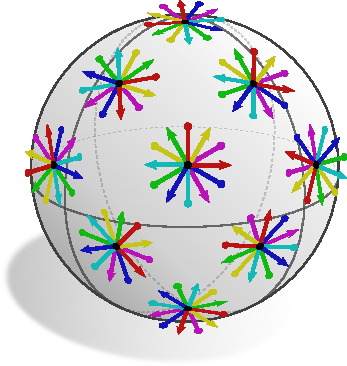
\includegraphics[width=.66\textwidth]{figures/G_structure_S2_1.pdf}
        \captionsetup{format=hang, width=.9\textwidth}
        \caption{\small
            $\SO2$-ساختار $\SOM$ روی کره ۲-بعدی $M=S^2$، که توسط دوران‌های سه‌بعدی عمومی در $\IsomSOM = \SO3$ حفظ می‌شود.
        }
        \label{fig:G_structure_S2_1}
    \end{subfigure}
    \hfill
    \begin{subfigure}[b]{0.48\textwidth}
        \centering
        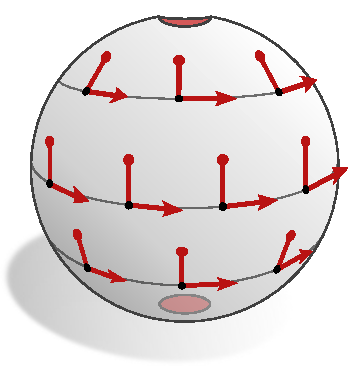
\includegraphics[width=.66\textwidth]{figures/G_structure_S2_2.pdf}
        \captionsetup{format=hang, width=.9\textwidth}
        \caption{\small
            $\{e\}$-ساختار $\eM$ روی یک کره ۲-بعدی سوراخ‌دار $M = S^2 \backslash \{n,s\}$، که توسط دوران‌های سمتی در $\IsomeM = \SO2$ حفظ می‌شود.
        }
        \label{fig:G_structure_S2_2}
    \end{subfigure}
    \vspace*{2ex}
    \caption{\small
        $G$-ساختارهای رایج زیربنای \lr{CNN}های کروی.
        موانع توپولوژیکی از کاهش گروه ساختاری کره ۲-بعدی فراتر از $G=\SO2$ جلوگیری می‌کنند.
        شکل~\ref{fig:G_structure_S2_1} $\SO2$-ساختار استاندارد روی $S^2$ را نشان می‌دهد، که با متریک جایگذاری (معادله~\eqref{eq:spherical_embedding_metric_explicit}) القا شده از حاصلضرب داخلی $\R^3$ مطابقت دارد.
        این ساختار تحت دوران‌ها در $\protect\IsomSOM = \SO3$ ناوردا است، که بر هموردایی دورانی کانولوشن $\GM$ متناظر دلالت دارد.
        توجه داشته باشید که تارهای $\GpM$ و $\GqM$ در نقاط مختلف $p$ و $q$ ایزومورف هستند اما نه به صورت کانونی -- به نظر می‌رسد رنگ‌های چارچوب در تصویر چنین ایزومورفیسمی را القا می‌کنند، با این حال، آنها به طور تصادفی انتخاب شده‌اند و هیچ معنایی ندارند.
        %
        شکل~\ref{fig:G_structure_S2_2} یک کره را نشان می‌دهد که در دو قطب متقابل سوراخ شده است.
        این کار کره را به یک استوانه توپولوژیکی $S^2 \backslash \{n,s\} \cong S^1\times(-\frac{\pi}{2},\frac{\pi}{2})$ با متریک شبه-کروی تبدیل می‌کند -- که اجازه یک کاهش کامل به یک گروه ساختاری بدیهی را می‌دهد.
        شکل، رایج‌ترین انتخاب از $\{e\}$-ساختار را نشان می‌دهد، که متناظر با چارچوب‌های راست‌هنجاری است که با شبکه مختصاتیِ مختصات کروی تراز شده‌اند؛ شکل~\ref{fig:spherical_equirectangular_1} را مقایسه کنید.
        از آنجا که این $\{e\}$-ساختار تحت دوران‌های سمتی حول محور قطبی ناوردا است، کانولوشن‌های $\GM$ متناظر $\protect\IsomeM = \SO2$-هموردا هستند.
        توجه داشته باشید که سوراخ کردن کره فقط وسیله‌ای برای پنهان کردن ناپیوستگی مدل‌ها در قطب‌ها است.
    }
    \label{fig:G_structures_S2_main}
\end{figure}